% !TEX program = xelatex
\documentclass[11pt, letterpaper]{exam}

\usepackage{amsmath}
\usepackage{amssymb}
\usepackage{graphicx}

\graphicspath{ {./images/} }

\renewcommand{\thesubpart}{(\roman{subpart})}
\renewcommand{\subpartlabel}{\thesubpart} % removes dot
\qformat{Exercise \thequestion: \hfill}

\newcommand{\tab}{\hspace*{.5cm}}
\newcommand{\includeimage}{\noindent\includegraphics[width=\linewidth]}


\title{Artificial Intelligence \\ Assignment  \\ Tutorial 4}
\author{Sudharshini Thangamurugan, 2577870 \\ Jeffrey Solomon, 2577386 \\ Ilya Senatorov, 2576798}
\date{May 14, 2019}

\begin{document}

  \maketitle

  \begin{questions}
  \setcounter{question}{8}
  \question

    \begin{parts}
    \part
    \begin{align*}
      &(P \lor (Q \iff R)) \land \neg (Q \to R) \\
      step 1 \tab &\equiv (P \lor ((Q \to R) \land (R \to Q))) \land \neg (Q \to R) \\
      step 2 \tab &\equiv (P \lor ((\neg Q \lor R) \land (\neg R \lor Q))) \land \neg (\neg Q \lor R) \\
      step 3 \tab & \equiv (P \lor ((\neg Q \lor R) \land (\neg R \lor Q))) \land (Q \land \neg R) \\
      simplify  & \equiv (P \land Q \land \neg R) \\
    \end{align*}

    \part
    \begin{align*}
      &\neg(P \iff Q) \to (Q \iff R) \\
      step 1 \tab &\equiv \neg((P \to Q) \land ( Q \to P)) \to ((Q \to R) \land (R \to Q)) \\
      step 2 \tab &\equiv \neg((\neg P \lor Q) \land (P \lor \neg Q)) \to ((\neg Q \lor R) \land (Q \lor \neg R)) \\
      step 2 \tab &\equiv ((\neg P \lor Q) \land (P \lor \neg Q)) \lor ((\neg Q \lor R) \land (Q \lor \neg R)) \\
      step 4 \tab &\equiv ((\neg P \lor Q \lor \neg Q \lor R) \land (\neg P \lor Q \lor Q \lor \neg R) \land (P \lor \neg Q \lor \neg Q \lor R) \land (P \lor \neg Q \lor Q \lor \neg R)) \\
      simplify & \equiv (\neg P \lor Q \lor \neg R) \land (P \lor \neg Q \lor R)
    \end{align*}
    \end{parts}

  \vspace{1em}
  \newpage
  \question
  \begin{parts}
    \part
    $ \Delta = \{\{\neg Q, R\},\{P,\neg R\},\{P,Q\},\{Q,R\},\{\neg P,\neg Q, R\},\{\neg R\}\} $ \\
    \includeimage{10a}

    \part
    $ \Delta = \{\{P,R\},\{\neg R, Q\},\{\neg Q, P\},\{Q,\neg P\},\{\neg Q, \neg P\}\} $ \\
    \includeimage{10b}

    \pagebreak
    \part
    $ \Delta = \{\{\neg P,R,S\},\{\neg R,\neg Q\},\{P,S,\neg Q\},\{\neg S,\neg Q\},\{\neg P,Q\},\{P,Q\}\} $ \\
    \includeimage{10c}

  \end{parts}

  \vspace{1em}

  \question
  \begin{parts}
    \part
      \begin{align*}
        & \Delta = \{\{\neg A,B,C\},\{\neg B,\neg C\},\{\neg A,\neg C,\neg D\},\{C,\neg D\},\{A,D\},\{A,\neg C,\neg D\}\} \\
        & \\
        & A \mapsto 0 \\
        &   \tab \{\{\neg B,\neg C\},\{C,\neg D\},\{D\},\{\neg C,\neg D\}\} \\
        &   \tab UP: D \mapsto 1 \\
        &     \tab\tab \{\{\neg B,\neg C\},\{C\}\{\neg C\}\} \equiv \square \\
        & A \mapsto 1 \\
        &   \tab \{\{B,C\},\{\neg B,\neg C\},\{\neg C,\neg D\},\{C,\neg D\}\} \\
        &   \tab B \mapsto 0 \\
        &     \tab\tab \{\{C\},\{\neg C,\neg D\},\{C,\neg D\}\} \\
        &     \tab\tab UP: C \mapsto 1 \\
        &       \tab\tab\tab \{\{C\},\{\neg D\},\{\neg D\}\} \\
        & Satisfiable: A = 1, B = 0, C = 1, D = 0
      \end{align*}
    \part
      \begin{align*}
        & \Delta = \{\{\neg  A,\neg B,C,\neg E\},\{\neg A,\neg B,C,E\},\{\neg A, B\},\{\neg B,A\},\{B,D\},\{B,C,\neg D\},\{\neg C\}\} \\
        & \\
        & UP: C \mapsto 0 \\
        & \{\{\neg  A,\neg B,\neg E\},\{\neg A,\neg B,E\},\{\neg A, B\},\{\neg B,A\},\{B,D\},\{B,\neg D\}\} \\
        & A \mapsto 0 \\
        & \{\{\neg B\},\{B,D\},\{B,\neg D\}\} \\
        &   \tab UP: B \mapsto 0 \\
        &   \tab\tab \{\{D\},\{\neg D\}\} \equiv \square \\
        & A \mapsto 1 \\
        & \{\{\neg B,\neg E\},\{\neg B,E\},\{B\},\{B,D\},\{B,\neg D\}\} \\
        &   \tab UP: B \mapsto 1 \\
        &   \tab\tab \{\{\neg B,\neg E\},\{\neg B,E\},\{B\},\{B,D\},\{B,\neg D\}\} \\
        &   \tab\tab \{\{\neg E\},\{E\}\} \equiv \square
      \end{align*}
      Not satisfiable since no combination of A and B will satisfy

  \end{parts}

  \question
    \begin{align*}
      & \Delta = \{\{A,B,C,D\},\{\neg A,\neg B\},\{\neg B, C\},\{\neg A,\neg D\},\{A,\neg D\},\{C,\neg D\},\{B, \neg C\},\{\neg B, C\},\{\neg A, C, D\}\} \\
      & A \mapsto 0 \\
      & \{\{B,C,D\},\{\neg B, C\},\{\neg D\},\{C,\neg D\},\{B, \neg C\},\{\neg B, C\}\} \\
      &   \tab UP: D \mapsto 0 \\
      &   \tab \{\{B,C\},\{\neg B, C\},\{B, \neg C\},\{\neg B, C\}\} \\
      &     \tab\tab B \mapsto 1 \\
      &     \tab\tab \{\{C\}\{\neg C\}\} \equiv \square
    \end{align*}

    \noindent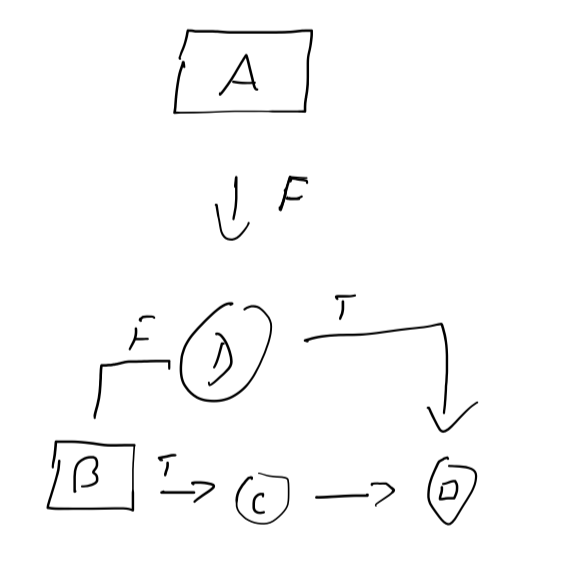
\includegraphics[width=4cm]{12a}

    Continuing where we left off with $A \mapsto 0, D \mapsto 1$ and adding the learned clause $\{A, \neg B\}$ \

    \begin{align*}
      & \{\{A, \neg B\},\{A,B,C,D\},\{\neg A,\neg B\},\{\neg B, C\},\{\neg A,\neg D\},\{A,\neg D\},\{C,\neg D\},\{B, \neg C\},\{\neg B, C\},\{\neg A, C, D\}\} \\
      & A \mapsto 0, D \mapsto 0 \\
      & \{\{A, \neg B\},\{B,C\},\{\neg B, C\},\{B, \neg C\},\{\neg B, C\}\} \\
      & \equiv \{\{\neg B\},\{B,C\},\{\neg B, C\},\{B, \neg C\},\{\neg B, C\}\} \\
      &   \tab\tab UP: B \mapsto 0 \\
      &   \tab\tab \{\{C\},\{\neg C\}\}
    \end{align*}

    \noindent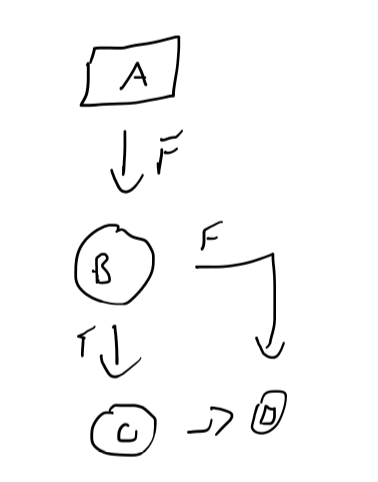
\includegraphics[width=4cm]{12b}

    Now, starting with the newly learned clause $\{A\}$ \\
    \begin{align*}
      & \{\{A\},\{A, \neg B\},\{A,B,C,D\},\{\neg A,\neg B\},\{\neg B, C\},\{\neg A,\neg D\},\{A,\neg D\},\{C,\neg D\},\{B, \neg C\},\{\neg B, C\},\{\neg A, C, D\}\} \\
      & UP: A \mapsto 1 \\
      & \{\{\neg B\},\{\neg B, C\},\{\neg D\},\{C,\neg D\},\{B, \neg C\},\{\neg B, C\},\{C, D\}\} \\
      &   \tab UP: B \mapsto 0 \\
      &   \tab \{\{\neg D\},\{C,\neg D\},\{\neg C\},\{C, D\}\} \\
      &     \tab\tab UP: C \mapsto 0 \\
      &     \tab\tab \{\{\neg D\},\{D\}\} \\
    \end{align*}

    \noindent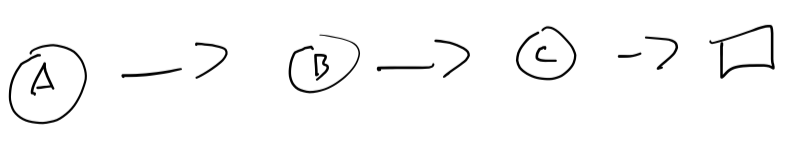
\includegraphics[width=8cm]{12c}

    This shows that this set of clauses is unsatisfiable.
  \end{questions}

\end{document}
